\documentclass[11pt]{article}

\usepackage{amsmath,amssymb,mathtools}
\usepackage[margin=1in]{geometry}
\usepackage{enumitem}
\usepackage{xcolor}
\usepackage{microtype}
\usepackage{graphicx}
\usepackage{tikz,float}
\usepackage{subcaption}
\usepackage{amsthm}
\usepackage{hyperref}
\usepackage{array}
\usepackage{pgfplots}

\usetikzlibrary{shapes.geometric, arrows.meta, positioning, calc, decorations.markings}
\tikzset{
	block/.style={rectangle, draw, text width=6em, text centered, rounded corners, minimum height=10mm},
	sum/.style={circle, draw, node distance=1.5cm},
	line/.style={draw, -{Stealth[length=2.5mm, width=1.5mm]}}
}

\usepgfplotslibrary{groupplots}
\pgfplotsset{compat=1.18}

\pgfplotsset{
	myaxes/.style={
		axis lines=middle,
		axis line style={-latex},
		grid=major,
		grid style={gray!15},
		minor grid style={gray!35},
		xlabel style={at={(ticklabel* cs:1)}, anchor=north west},
		ylabel style={at={(ticklabel* cs:1)}, anchor=south east},
		every axis plot/.append style={thick}
	},
	myplotstyle/.style={
		width=14cm,
		height=7cm,
		axis lines=middle,
		axis line style={-Stealth},
		grid=both,
		minor tick num=1,
		major grid style={draw=gray!30},
		minor grid style={draw=gray!15},
		tick label style={font=\small, fill=white, inner sep=1.5pt},
		xlabel={$t$},
		ylabel={$x(t)$},
		xlabel style={anchor=north east, font=\small},
		ylabel style={anchor=south east, font=\small},
		samples=401,
	}
}

\newtheoremstyle{mynote}
{6pt}      % Space above
{6pt}      % Space below
{}          % Body font (normal, not italic)
{}          % Indent amount
{\bfseries} % Theorem head font
{.}         % Punctuation after theorem head
{.5em}      % Space after theorem head
{}          % Theorem head spec
\theoremstyle{mynote}
\newtheorem{definition}{Definition}
\newtheorem{proposition}{Proposition}
\newtheorem{example}{Example}
\newtheorem{remark}{Remark}
\newtheorem{theorem}{Theorem}
\newtheorem{corollary}{Corollary}

\newcommand{\T}{\mathcal{T}}
\newcommand{\R}{\mathbb{R}}
\newcommand{\Z}{\mathbb{Z}}
\newcommand{\C}{\mathbb{C}}
\newcommand{\conv}{\ast}
\newcommand{\dt}{\,\dd t}
\newcommand{\dd}{\mathrm{d}}
\newcommand{\imp}{\delta}
\newcommand{\sinc}[1]{\frac{\sin(\pi #1)}{\pi #1}}


\DeclareMathOperator{\rect}{rect}
\DeclareMathOperator{\Ev}{Ev}
\DeclareMathOperator{\Od}{Od}
\DeclareMathOperator{\sgn}{sgn}
\DeclareMathOperator{\step}{u}
\DeclareMathOperator{\tri}{tri}

\begin{document}
	% Reset figure counter for this lecture
	\renewcommand{\thefigure}{18.\arabic{figure}}
	
	% --- TITLE BLOCK ---
	\thispagestyle{empty}
	\noindent
	\begin{tabular*}{\textwidth}{l @{\extracolsep{\fill}} r}
		\textbf{Signals and Systems} & \textbf{Lecture 18} \\
		\textit{Dr. Ghandi Manasra and Ahmed Rabei} & \textit{Fall 2025} \\
	\end{tabular*}
	\hrule
	\vspace{0.4cm}
	\begin{center}
		\Large\textbf{Lecture 18: The Frequency Response of LTI Systems}
	\end{center}
	\vspace{0.4cm}
	
	\section*{Reference}
	Oppenheim \& Willsky, \textit{Signals and Systems}, Chapter 6, Section 6.2
	
	\section*{Review of Lecture 17}
	\begin{itemize}[noitemsep]
		\item Fourier transform represented in polar form: $X(j\omega) = |X(j\omega)|e^{j\angle X(j\omega)}$
		\item Magnitude tells us "what frequencies" are present
		\item Phase tells us "how frequencies align in time"
		\item Phase often more important than magnitude for signal structure
		\item Today: applying magnitude/phase concepts to LTI systems
	\end{itemize}

\section*{18.1 Frequency Response of LTI Systems}

For an LTI system with impulse response $h(t)$, the frequency response is:
\[
H(j\omega) = \int_{-\infty}^{\infty} h(t) e^{-j\omega t} \dd t
\]

The frequency response can be written in polar form:
\[
H(j\omega) = |H(j\omega)|e^{j\angle H(j\omega)}
\]

Since the output spectrum is $Y(j\omega) = H(j\omega)X(j\omega)$, we can express the output magnitude and phase as:
\begin{itemize}[noitemsep]
	\item \textbf{Output Magnitude:} $|Y(j\omega)| = |H(j\omega)| \cdot |X(j\omega)|$ (Magnitudes multiply)
	\item \textbf{Output Phase:} $\angle Y(j\omega) = \angle H(j\omega) + \angle X(j\omega)$ (Phases add)
\end{itemize}

This shows how an LTI system modifies both the magnitude and phase of the input signal's spectrum.

\begin{figure}[H]
	\centering
	
	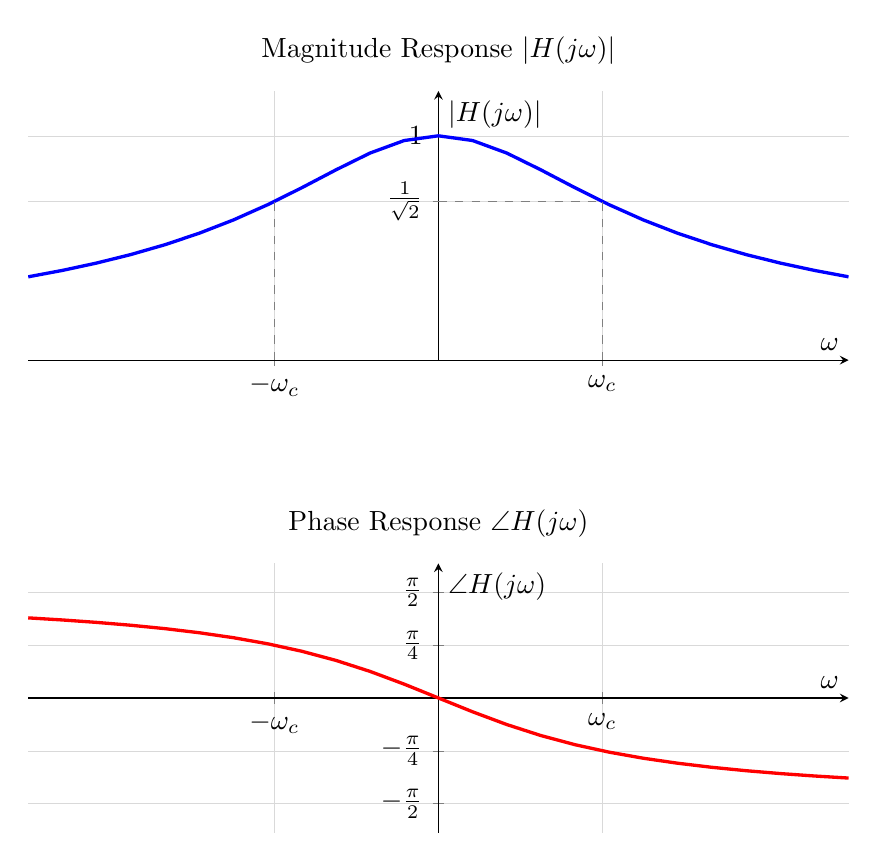
\begin{tikzpicture}
		% Define a common style
		\pgfplotsset{
			lpf a/.style={
				width=12cm, height=5cm,
				axis lines=middle, xlabel={$\omega$},
				xmin=-5, xmax=5,
				xtick={-2, 2},
				grid=major, grid style={line width=.1pt, draw=gray!30},
				no marks,
			}
		}
		
		% Top plot: Magnitude
		\begin{scope}[yshift=6cm]
			\begin{axis}[
				lpf a,
				title={Magnitude Response $|H(j\omega)|$},
				ylabel={$|H(j\omega)|$},
				ymin=0, ymax=1.2,
				xticklabels={$-\omega_c$, $\omega_c$},
				ytick={0.707, 1},
				yticklabels={$\frac{1}{\sqrt{2}}$, $1$},
				]
				\addplot[blue, very thick, domain=-5:5] {1 / sqrt(1 + (x/2)^2)};
				\draw[dashed, gray] (axis cs:2,0) -- (axis cs:2, {1/sqrt(2)});
				\draw[dashed, gray] (axis cs:-2,0) -- (axis cs:-2, {1/sqrt(2)});
				\draw[dashed, gray] (axis cs:0,{1/sqrt(2)}) -- (axis cs:2, {1/sqrt(2)});
			\end{axis}
		\end{scope}
		
		% Bottom plot: Phase
		\begin{scope}[yshift=0cm]
			\begin{axis}[
				lpf a,
				title={Phase Response $\angle H(j\omega)$},
				ylabel={$\angle H(j\omega)$},
				ymin=-2, ymax=2,
				xticklabels={$-\omega_c$, $\omega_c$},
				ytick={-1.57, -0.785, 0.785, 1.57},
				yticklabels={$-\frac{\pi}{2}$, $-\frac{\pi}{4}$, $\frac{\pi}{4}$, $\frac{\pi}{2}$},
				]
				% --- FIXED LINE ---
				% Convert atan output (degrees) to radians by multiplying by pi/180
				\addplot[red, very thick, domain=-5:5] {-atan(x/2) * pi/180};
			\end{axis}
		\end{scope}
	\end{tikzpicture}
	









	\caption{Magnitude and phase response of an LTI system.}
	\label{fig:frequency_response_representation}
\end{figure}

\section*{18.2 Linear Phase Systems}

Consider a system that is a pure time delay: $y(t) = x(t-t_d)$. Its frequency response is:
\[
H(j\omega) = e^{-j\omega t_d}
\]

This has:
\begin{itemize}[noitemsep]
	\item \textbf{Magnitude Response:} $|H(j\omega)| = 1$ (all-pass filter)
	\item \textbf{Phase Response:} $\angle H(j\omega) = -\omega t_d$ (linear in frequency)
\end{itemize}

\begin{definition}
	A system has \textbf{linear phase} if its phase response is of the form $\angle H(j\omega) = -\alpha\omega$. All frequency components experience the same time delay $\alpha$, preserving the signal shape perfectly.
\end{definition}

\begin{figure}[H]
	\centering
	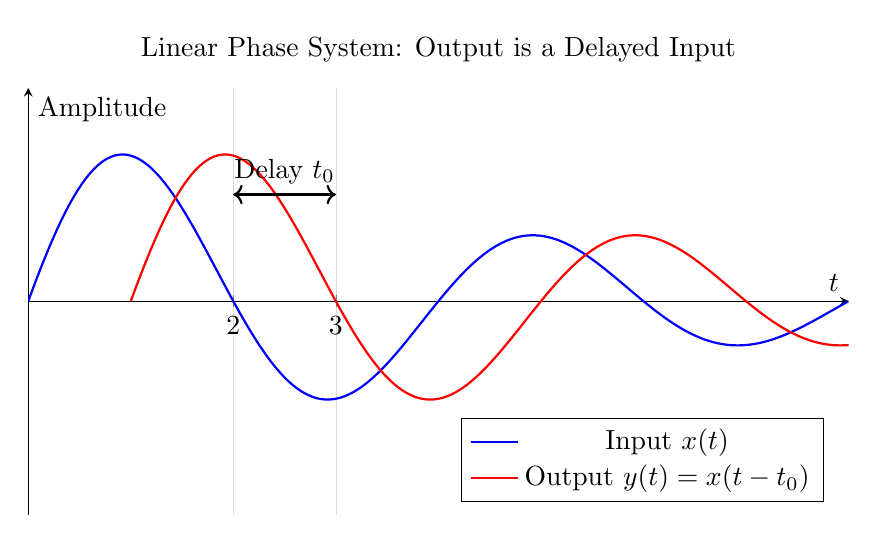
\begin{tikzpicture}
	\begin{axis}[
		width=12cm,
		height=7cm,
		title={Linear Phase System: Output is a Delayed Input},
		xlabel={$t$},
		ylabel={Amplitude},
		axis lines=middle,
		xmin=0, xmax=8,
		ymin=-1.2, ymax=1.2,
		xtick={2,3},
		ytick=\empty,
		grid=major,
		grid style={line width=.1pt, draw=gray!30},
		legend pos=south east,
		no marks,
		]
		\addplot[blue, thick, domain=0:8, samples=200] {sin(deg(2*pi*x/4)) * exp(-0.2*x)};
		\addlegendentry{Input $x(t)$};
		
		\addplot[red, thick, domain=1:8, samples=200] {sin(deg(2*pi*(x-1)/4)) * exp(-0.2*(x-1))};
		\addlegendentry{Output $y(t) = x(t-t_0)$};
		
		\draw[<->, thick] (axis cs:2,0.6) -- (axis cs:3,0.6) node[midway, above] {Delay $t_0$};
	\end{axis}
\end{tikzpicture}











	\caption{Linear phase system preserves signal shape with constant delay.}
	\label{fig:linear_phase_system}
\end{figure}

\paragraph{Key Properties:}
\begin{itemize}[noitemsep]
	\item Output: $y(t) = x(t - \alpha)$ (perfect shape preservation)
	\item Constant group delay across all frequencies
	\item No phase distortion
\end{itemize}

\section*{18.3 Group Delay}

Most practical systems have nonlinear phase. The \textbf{group delay} characterizes the delay experienced by signal envelopes:

\begin{definition}
	The \textbf{group delay} is:
	\[
	\tau_g(\omega) = -\frac{d}{d\omega}\{\angle H(j\omega)\}
	\]
\end{definition}

\subsection*{18.3.1 Phase Distortion}

When group delay varies with frequency, different frequency components experience different delays, causing \textbf{phase distortion}. This distorts signal shape even with flat magnitude response.

\begin{figure}[H]
	\centering
	\resizebox{0.8\textwidth}{!}{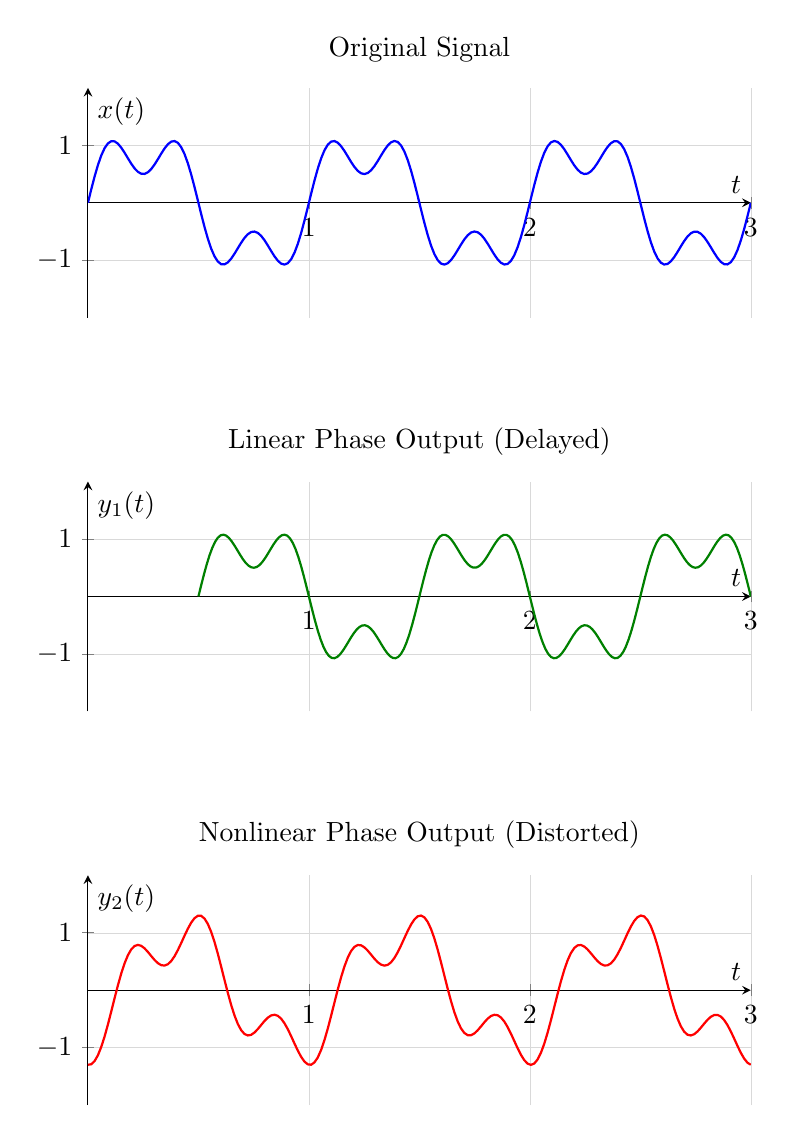
\begin{tikzpicture}
	% Define a common style
	\pgfplotsset{
		phase b/.style={
			width=10cm, height=4.5cm,
			axis lines=middle, xlabel={$t$},
			xmin=0, xmax=3, ymin=-2, ymax=2,
			xtick={1,2,3}, ytick={-1,1},
			grid=major, grid style={line width=.1pt, draw=gray!30},
			no marks,
			samples=200,
		}
	}
	\begin{scope}[yshift=10cm]
		\begin{axis}[phase b, title={Original Signal}, ylabel={$x(t)$}]
			\addplot[blue, thick, domain=0:3] {sin(deg(2*pi*x)) + 0.5*sin(deg(6*pi*x))};
		\end{axis}
	\end{scope}
	\begin{scope}[yshift=5cm]
		\begin{axis}[phase b, title={Linear Phase Output (Delayed)}, ylabel={$y_1(t)$}]
			\addplot[green!50!black, thick, domain=0.5:3] {sin(deg(2*pi*(x-0.5))) + 0.5*sin(deg(6*pi*(x-0.5)))};
		\end{axis}
	\end{scope}
\begin{axis}[phase b, title={Nonlinear Phase Output (Distorted)}, ylabel={$y_2(t)$}]
	\addplot[red, thick, domain=0:3] {sin(deg(2*pi*x - 45)) + 0.5*sin(deg(6*pi*x - 90))};
\end{axis}
	
\end{tikzpicture}








}
	\caption{Phase distortion demonstration: linear vs. nonlinear phase systems.}
	\label{fig:phase_distortion_demo}
\end{figure}

\section*{18.4 Phase Distortion Demonstration}

Consider a signal with fundamental and third harmonic:
\[
x(t) = \sin(2\pi t) + 0.5\sin(6\pi t)
\]

When this passes through:
\begin{enumerate}[noitemsep]
	\item \textbf{Linear phase system:} All components delayed equally, shape preserved
	\item \textbf{Nonlinear phase system:} Different delays cause shape distortion
\end{enumerate}

\begin{figure}[H]
	\centering
	\resizebox{0.8\textwidth}{!}{\begin{tikzpicture}
	\begin{groupplot}[
		group style={group size=1 by 3, vertical sep=8mm},
		width=\linewidth,          % unified width for all three plots
		height=0.28\textheight,      % choose a proportional height
		grid=major,
		grid style={line width=.1pt, draw=gray!30},
		axis lines=middle,
		no marks
		]
		
		% 1) Harmonic Signal
		\nextgroupplot[
		title={Harmonic Signal: $x(t) = \sin(2\pi t) + 0.5\sin(6\pi t)$},
		xlabel={$t$}, ylabel={$x(t)$},
		xmin=0, xmax=2, ymin=-1.5, ymax=2,
		xtick={0,0.5,1,1.5,2},
		ytick={-1.5,-1,-0.5,0.5,1,1.5}
		]
		\addplot[blue, very thick, domain=0:2, samples=200] {sin(deg(2*pi*x)) + 0.5*sin(deg(6*pi*x))};
		\node[anchor=west, text width=7cm] at (axis cs:0.7, 1.4)
		{Fundamental: $\omega_0 = 2\pi$ rad/s \ 3rd Harmonic: $3\omega_0 = 6\pi$ rad/s};
		
		% 2) Phase Response (FIXED xmax and linear function)
		\nextgroupplot[
		title={Phase Response Comparison},
		xlabel={$\omega$}, ylabel={$\angle H(j\omega)$},
		xmin=0, xmax=20, % <-- FIXED: Was 7, now 20 (must be > 6*pi)
		ymin=-20, ymax=2,
		xtick={2*pi,6*pi}, xticklabels={$\omega_0$,$3\omega_0$},
		legend pos=north east
		]
		% FIXED: Changed from -0.2*x to -0.4*x to match the t_0=0.4 delay in Plot 3
		\addplot[green!50!black, thick, domain=0:20] {-0.4*x}; 
		\addlegendentry{Linear Phase ($\phi = -0.4\omega$)};
		\addplot[red, thick, domain=0:20, samples=200] {-0.1*x - 0.05*x^2};
		\addlegendentry{Nonlinear Phase};
		\draw[dashed, gray] (axis cs:{2*pi},-3) -- (axis cs:{2*pi},2);
		\draw[dashed, gray] (axis cs:{6*pi},-3) -- (axis cs:{6*pi},2);
		
		% 3) Output Comparison (FIXED syntax and nonlinear example)
		\nextgroupplot[
		title={Output Comparison},
		xlabel={$t$}, ylabel={$y(t)$},
		xmin=0, xmax=3, ymin=-3, ymax=2,
		xtick={1,2,3}, ytick={-1.5,-1,-0.5,0.5,1,1.5},
		legend pos=south west
		]
		% This plot now correctly corresponds to the green line in Plot 2
		\addplot[green!50!black, thick, domain=0:3, samples=200] {sin(deg(2*pi*(x-0.4))) + 0.5*sin(deg(6*pi*(x-0.4)))};
		\addlegendentry{Linear Phase Output (Delayed by $t_0=0.4$)};
		
		% FIXED: Corrected sin(deg(...)) syntax
		% FIXED: Changed -135 to -200 to be TRULY nonlinear (3*(-45) != -200)
		\addplot[red, thick, domain=0:3, samples=200] {sin(deg(2*pi*x) - 45) + 0.5*sin(deg(6*pi*x) - 200)};
		\addlegendentry{Nonlinear Phase Output (Distorted)};
		
	\end{groupplot}
\end{tikzpicture}}
	\caption{Effect of phase distortion on a signal with multiple harmonics.}
	\label{fig:harmonic_phase_distortion}
\end{figure}

\newpage
\section*{Summary and Next Lecture}
	\begin{itemize}[noitemsep]
		\item Magnitude response $|H(j\omega)|$ controls frequency amplification and attenuation
		\item Phase response $\angle H(j\omega)$ controls time alignment of frequency components
		\item Linear phase corresponds to pure time delay with no shape distortion
		\item Group delay $\tau_g(\omega) = -\frac{d}{d\omega}\{\angle H(j\omega)\}$ characterizes signal envelope delay
		\item Nonlinear phase causes non-constant group delay and phase distortion
		\item \textbf{Next time:} Trade-offs between ideal and non-ideal filters
	\end{itemize}

\end{document}
